\chapter{Tool Refactoring Methodology}%
\label{methodology}

\section{Architectural Analysis of Packages within RMT}

To understand the operational dynamics of RMT, it is imperative to analyze the codebase, specifically the various packages. The initial phase of the updating process involves discerning the functionality of different code segments to determine whether to undertake a code refactoring or a comprehensive service rewrite.

\subsection{Intermediary Sevice Packages Analisys}
\label{sub-intermediary-packages}
The intermediary service is systematically divided into four main packages, each comprising functionalities. The first functionality involves the management of refactoring projects. The second pertains to the facilitation of inter-service communication. The third serves as a service discovery mechanism by registering the addresses of all ancillary services to enable seamless subsequent communications. They are illustrated by the package diagram shown in \Cref{fig-package-intermediary}.

\begin{figure}[ht!]
\SetCaptionWidth{\textwidth}
\caption{Intermediary Service Package Diagram}
\label{fig-package-intermediary}
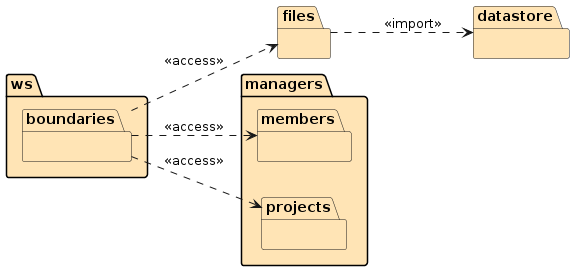
\includegraphics[width =\textwidth, scale=0.2]{Chapter-4/Figures/intermediary-service.png}
\SourceOrNote{Own authorship (2024)}
\end{figure}
\FloatBarrier

The package \verb|datastore| encompasses all configuration files pertinent to the database pool and the connection configuration.

The package \verb|files| contains repository files for database interactions, facilitating queries, insertions, and additional data manipulations.

Within the manager package, the entire outbound logic refers to the refactoring process and the discovery of services, encompassing all related requests for refactoring and generating metrics in the package \verb|managers.projects| and registering the services in the package \verb|managers.members|.

For handling communication, the \verb|ws.boundaries| package includes the controller configurations. Within this package, business logic is assigned to the persistence and querying of projects and dispatching requests to other services. Consequently, this package must access the \verb|managers| and \verb|files| packages.

\subsection{Detection Service Package Analisys}

The detection service is arranged into six main packages, the core functionalities of which are periodically communicated with the intermediary service to ensure registration with the service discovery mechanism. Moreover, interfaces have been developed to analyze the source code for potential refactoring candidates, and interfaces have been designed to execute refactoring on projects identified as containing such candidates. The package diagram displayed in \Cref{fig-package-detection} illustrates them.
\begin{figure}[ht!]
\SetCaptionWidth{\textwidth}
\caption{Detection Service Package Diagram}
\label{fig-package-detection}
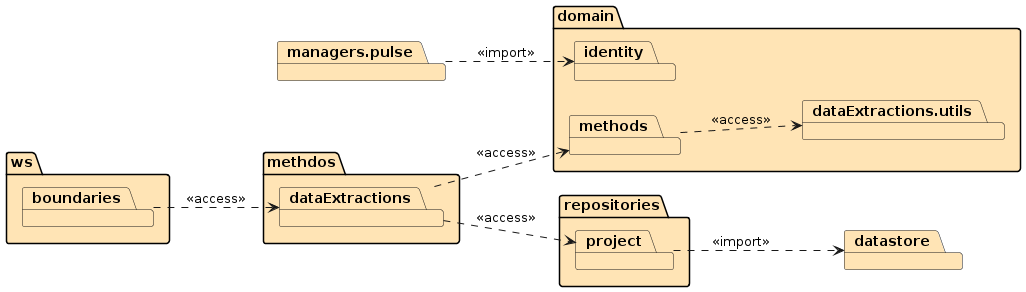
\includegraphics[width =\textwidth, scale=1.0]{Chapter-4/Figures/detection-service.png}
\SourceOrNote{Own authorship (2024)}
\end{figure}
\FloatBarrier

The package \verb|datastore| is configured with identical database parameters to those defined in \cref{sub-intermediary-packages}.

The Package \verb|repository.project| has logic to manipulate the database where projects are saved and retrieved for unrefactored and refactored projects. The database configuration, such as the address and ports, is imported from the \verb|datastore| package.

The package \verb|methos.dataExtractoins| includes preconfigured interfaces for implementing various code extraction methods. The Abstract Syntax Tree is implemented as the extraction method for the refactoring processes within the RMT. Following the code transformation into an Abstract Syntax Tree (AST), the service accesses the files within the \verb|domain.mehtos| to perform its designated function.

The package \verb|managers.pulse| includes the configuration for the service registry, sending requests every minute as proof of life to the intermediary service, and it can receive requests. The information, such as the address and port sent from the service, is retrieved from the package \verb|domain.identity|.

The interfaces for candidates searching and refactoring projects are in the \verb|domain.methdos| has interfaces to implement and extend the tool refactoring options. As the current methods implement the Abstract Syntax Tree as an extraction method, the \verb|doamin.dataExtraction.utils| package has methods to facilitate the manipulation of the AST.

To start refactoring, the controllers must receive an HTTP request on the \verb|ws.boundaries| that distributes the request based on its URL path among the other class functions. 

\subsection{Metrics Service Package Analisys}


\begin{figure}[ht!]
\SetCaptionWidth{\textwidth}
\caption{Metrics Service Package Diagram}
\label{fig-package-metrics}
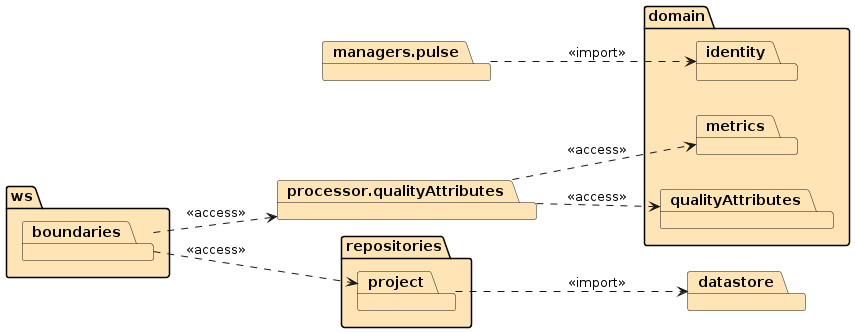
\includegraphics[width =\textwidth, scale=1.0]{Chapter-4/Figures/metrics-service.png}
\SourceOrNote{Own authorship (2024)}
\end{figure}
\FloatBarrier

Consistent with the preceding two services, the \verb|datastore| is the repository for all database configuration settings.

To access the unrefactored and refactored projects, the package \verb|repository.project| has all the logic queries to the database using the information provided by the \verb|datastore| package.

Correspondingly to the previous service, the package \verb|managers.pulse| encompasses the comprehensive logic required for registration within the service discovery mechanism. This service adheres stringently to all the specifications delineated in the detection service.

Similarly to the detection service, the \verb|processor.qualityAttributes| has the interfaces to implement different methods of measuring code metrics and quality attributes. The interfaces' logic and calculations are in the \verb |domain.metrics| and \verb|domain.qualityAttribute| packages.

The classes with logic and calculations for generating metrics are in the \verb|domain.metrics| package; for now, they are hardcoded, implementing the CK module created by \textcite{ck}; however, the interface is designed to integrate additional metrics generation methodologies. In the \verb|domain.qualityAttributes| package is located in the calculations for quality attributes, such as maintainability, readability, etc.

Consistent with previous services, the \verb|ws.boundaries| packages serve as the access point for service functionalities. They coordinate computations by interfacing with the database to retrieve project data and invoke methods within the \verb|processor.qualityAttributes| packages, thereby generating metrics and quality attributes.
 
\section{Inicio - Criação de testes}

Me basear no fowler que presa por ter teste unitário antes de modificar para que se possa permanecer o comportamento.

\subsection{Metrics Calculation Service}

\subsection{Detection And Refactoring}

\section{Refatoracao}

\subsection{Refactoring And Metrics Manager Service}

\subsection{Detection And Refactoring Service}

\subsection{Metrics Calculation Service}

\section{Teste da ferramenta}